\chapter{Configuration}\label{cha:configuration}
XCSoar est un calculateur de vol très configurable et peut être paramétré pour répondre aux préférences des différents utilisateurs. Ce chapitre décrit le paramétrage et les options disponibles.

\section{Champ d'application de la configuration}
Il y a plusieurs façons de paramétrer XCSoar:
\begin{itemize}

\item Modification des paramètres. Ce sont les paramètres les plus couramment modifiés par les utilisateurs. Ce document en explique le fonctionnement en détail.
\item Changement de la langue, ou juste pour modifier le libellé du texte dans l'interface utilisateur.
\item Changement des affectations des boutons et des menus. Ceci permet de changer le contenu et la structure des menus.
\item Changement et ajout d'actions lors de la survenue d'évènements gérés par le calculateur.
\item Définition du temps d'affichage des messages d'état et des sons associés lors de l'affichage de ces messages.
\end{itemize}
La description de tout ceci en détail va au delà du contenu d'un manuel utilisateur. Pour plus d'information l'utilisateur peut parcourir le wiki d'XCSoar. \url{http://www.xcsoar.org/trac/wiki}
%Describing all of these in a detail level like a reference manual would 
%do is beyond the scope of this document. The user is referred to browse 
%through the XCSoar Wiki for more details. 
%\url{http://www.xcsoar.org/trac/wiki}

\section{Modification des paramètres}

Il y a un grand nombre de paramètres de configuration qui peuvent être modifiés à l'aide du menu:
\begin{quote}
\bmenu{Config.}\blink\bmenu{Config. 1/3}\blink\bmenu{Config. 2/3}\blink\bmenu{Options Système}
\end{quote}
Le paramètrage est accessible à l'aide d'un menu à 2 niveaux ou séquentiellement avec les boutons flèche droite ou gauche.

\begin{center}
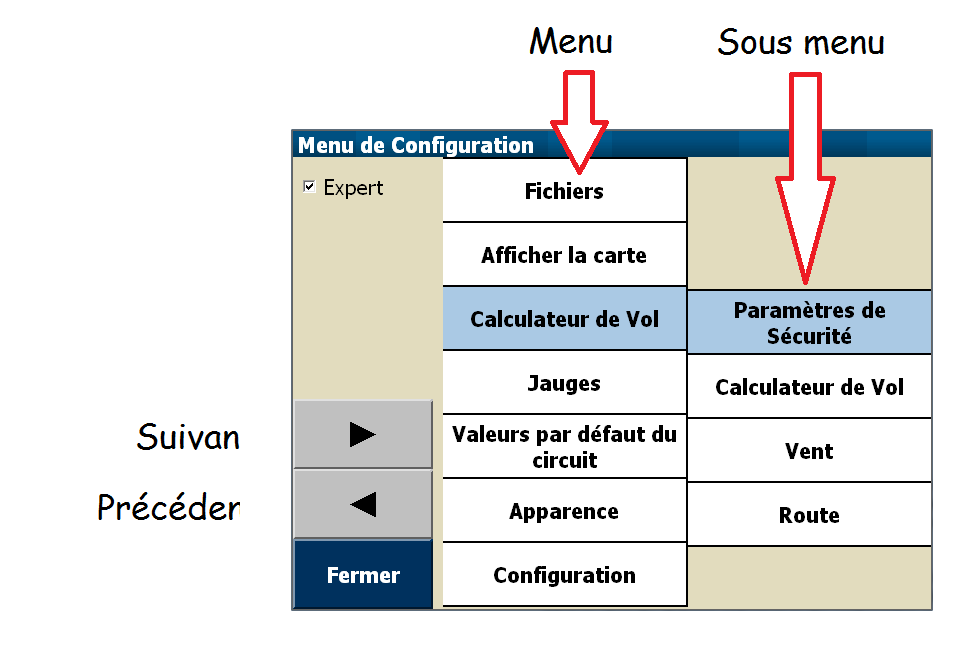
\includegraphics[angle=0,width=1.0\linewidth,keepaspectratio='true']{figures/config-menu.png}
\end{center}

Il est fortement recommandé de ne pas changer ces paramètres en vol. \warning Tout changement de paramétrage doit se faire au sol afin de pouvoir en vérifier les effets sur le calculateur. 

Le menu Options Système comporte de nombreuses pages. Une fois qu'une page a été modifiée, le passage à une autre page se fait soit avec  \bmenu{Fermer} soit en passant à la suivante ou à la précédente. Sur Altair utiliser PWR/ESC. Une seconde pression sur \bmenu{Fermer} permet de retourner à l'écran de navigation.

\tip Une fois que vous avez paramétré l'ensemble du logiciel, sauvegardez votre fichier profil sur un autre support (clé USB, PC, ...) afin de pouvoir tout récupérer si la mémoire de votre appareil venait à être effacée.

Voir le chapitre~\ref{cha:data-files} pour une description des formats des fichiers de paramétrage. Quand aucun fichier est utilisé, le champ peut être laissé vide. Les noms de fichiers dans les formulaires sont filtrés par leur extension (ex: .txt, .cup,...). Ceci rend beaucoup plus facile leur recherche et leur sélection.

Le menu principal de paramétrage (Options Systèmes) peut-être utilisé en mode "Basique" ou "Expert" à l'aide de la case à cocher en haut à gauche de la page. \sketch{figures/config-expert.png} En mode "Basique", une grande partie des paramètres les moins souvent utilisés sont cachés. Dans la suite de ce document, tout les paramètres marqués d'un astérisque ne sont visibles qu'en mode "Expert".


%%%%%%%%%%%%%%%%%%
\section{Fichiers / Fichiers}
Ce panel permet de définir la plupart des fichiers qui doivent être utilisés lors d'un vol dans une nouvelle région.

\begin{description}
\item[Chemin d'accès aux données d'XCSoar]  (PATH) Chemin principal de stockage des données utilisées par XCSoar sur votre appareil: disque dur, carte SD, mémoire statique de PDA,...
\item[Carte]  Nom du fichier de la carte (.XCM) contenant des informations d'altitude du relief, topographie et optionnellement des points de virage et des espaces aériens.
\item[Waypoints]  Fichier principal de points de virage. Si ce champ est vide, les points de virages sont chargés à partir de la carte de relief (.xcm), si elle existe.
\item[Autres wpts.*]  Fichier secondaire de points de virage. Il peut être utilisé pour ajouter les points de virage d'une compétition.
\item[Waypoints spéc.*]  Fichier de points de virage spéciaux: points utiles pour les calculs d'arrivée, repères d'ascendances fiables (usines, centrales thermiques,...), col en montagne,...
\item[Espaces aériens] Fichier principal des espaces aériens. Si ce champ est vide, les espaces aériens sont chargés à partir de la carte de relief (.xcm), si elle existe.
\item[Autres esp. aér.*]  Fichier secondaire des espaces aériens.
%\item[Terrain file*]  The name of the file containing digital elevation
%  terrain data.  Typically left blank, because terrain is loaded from the map
%  file.
%\item[Topography file*]  Specifies the file defining the topographical features.
%The topography file defines the map topography in terms of points, lines
%and areas with optional labels.  Typically left blank, because topography is
%loaded from the map file.
\item[Détails wpts.*]  Le fichier de terrains reconnus peut contenir des informations officielles ou non. Ces points de virage détaillés permettent d'avoir les informations sur des terrains d'aviation ou des terrains vachables reconnus ou bien édités par le pilote lui même.
\end{description}

Les fichiers d'espace aériens décrivent les "espaces aériens d'usage spécial" (“Special Use Airspace”). Jusqu'à deux fichiers peuvent être définis: le premier en tant que fichier SUA principal, le second dédié aux espaces aériens impactés par des NOTAM. 
Le fichier des espaces aérien Français mis à jour par la FFVV est disponible ici \url{http://www.ffvvespaceaerien.org/?page_id=412}

\sketch{figures/config-site.png}

Le format de fichier XCM est celui recommandé pour l'utilisation de XCSoar. La version précédente (XCSoar V5.x) nécessitait des fichiers séparés pour le relief et la topographie.

Quand la carte au format XCM est utilisée, elle contient les informations de relief, de topographie et en option, elle peut aussi contenir des points de virages et les espaces aériens. Dans ce cas les champs des fichiers "Waypoints" et "Espaces aériens" peuvent être laissés vides, les points de virages et les espaces aériens sont alors chargés à partir de la carte XCM. Si la carte au format XCM utilisée comporte des points de virages et/ou des espaces aériens, l'utilisateur peut toujours définir ses fichiers de points de virage et d'espaces aériens; ceux-ci seront pris en compte à la place des informations contenues dans la carte XCM.

See Section~\ref{sec:map} for more details on map files.


%%%%%%%%%%%%%%%%%%
\section{Afficher la carte / Orientation}\label{sec:map-projection}

Ce panel permet de choisir, en autre, le l'orientation de la carte en vol.

\begin{description}
\item[Orientation Transition/Spirale]  \label{conf:orientation} Ceci détermine la rotation de l'écran par rapport au planeur, en fonction du mode d'affichage courant. \\
  {\bf Route en haut}: La carte mobile sera montrée de telle façon que la trajectoire du planeur soit dirigée vers le haut de l'écran. Le symbole de la flèche de la boussole pointe vers le nord vrai. Le symbole du planeur peut ne pas pointer vers le haut car il pointe vers son cap calculé qui tient compte de la dérive due au vent.\\ 
  \sketch{figures/config-map_projection.png}
  {\bf Nord en haut}: La carte est toujours orientée Nord vrai en haut de l'écran, le symbole du planeur pivote vers la direction de sa route corrigée de la dérive due au vent.\\
  {\bf Cible en haut}: La carte est orientée de façon à ce que l'objectif courant soit en haut de l'écran.
\item[Zoom en spirale]  \label{conf:circlingzoom} Permet de choisir si des valeurs de zoom en spirale et en transition peuvent être différentes. Si activé, alors la carte sera zoomée  automatiquement lors de la mise en spirale et sera dézoomée en sortie de spirale.
\item[Réf. de décalage carte] Le déplacement de la carte peut être ajusté afin d'améliorer sa lecture. Ce choix n'est possible qu'en vol ou en mode simulation après quelque minutes.\\
  {\bf Aucun}: Pas d'ajustement. \\
  {\bf Route}: Utiliser la moyenne récente de la route au sol comme référence.\\
  {\bf Objectif}: Utiliser le point de virage cible comme base.
\item[Max. dist. zoom auto]  \label{conf:gliderposition} Définit la position en pourcentages du planeur sur l'écran à partir du bord de l'écran.
\item[Max. auto zoom distance]  Distance maxi à l'écran en zoom automatique.
\end{description}


%%%%%%%%%%%%%%%%%%
\section{Afficher la carte / Éléments}\label{sec:map-elements}

Ce panel liste des éléments optionnels superposés à la carte.

\begin{description}
\item[Trace sol]  Affiche la trace au sol (projection sur le sol). "Auto" permet d'afficher la trace sol si elle est significativement différente du cap à suivre.
\item[Traffic FLARM]  \label{conf:flarm-on-map} Permet d'afficher le traffic FLARM sur la carte.
\item[Longueur Trace*] \label{conf:snailtrail} Longueur de la trace sol derrière le planeur.\\
\sketch{figures/config-map_elements.png}
  {\bf Off}: pas de trace. \\
  {\bf Long}:trace longue (environ 60 minutes). \\
  {\bf Court}:trace courte (environ 10 minutes). \\
  {\bf Complet}: trace du vol complet.
\item[Dérive Compensée en spirale*] \label{conf:traildrift} Détermine si la trace est compensée par rapport à la dérive due au vent en spirale. Sur Off, il n'y a pas de compensation.
\item[Type de la trace*] \label{conf:snailtype} Type d'affichage de la trace. \\
  {\bf Vario \#1}: En zone ascendante la trace est épaisse et verte. En zone descendante elle est rouge et fine. Elle est grise en Vz nulle.\\
  {\bf Vario \#2}: En montée la couleur de la trace passe du orange au rouge. En descente, elle passe du bleu clair au bleu foncé. Avec une Vz nulle, la trace est jaune.\\
  {\bf Altitude}: La couleur de la trace varie en fonction de l'altitude.
\item[Épaississement de la trace*] \label{conf:trailscaled} Sur ON, l'épaisseur de la trace en spirale est proportionnelle à la valeur du vario.
\item[Indicateurs du détour*]  En transition, ceci permet d'afficher des petites marques (chiffres) devant le nez du planeur. C'est la distance additionnelle, en pourcentages, si vous allez jusqu'à la position de la marque et ensuite directement vers le point de virage cible, par rapport à la distance minimum entre votre position et la cible.
\item[Symbole du planeur*]  Choix du symbole représentant l'aéronef. \\
  {\bf Simple}: Représentation simplifiée; le planeur est noir avec un contour blanc.\\
  {\bf Simple (large)}: comme "Simple" mais plus grand pour une meilleure visibilité sur de petits écrans.\\
  {\bf Détaillé}: Représentation détaillée.\\
 {\bf Delta plane}: Représentation simplifiée d'un Delta plane (filaire, blanc, contour noir) .\\
 {\bf Parapente}: Représentation simplifiée d'un parapente (filaire, blanc, contour noir) .
\item[Flèche de vent*]  Choix de la représentation du vent sur la carte. \\
  {\bf Tête de flèche}: La tête d'une flèche. \\
  {\bf Flèche complète}: La tête d'une flèche avec une ligne pointillée.
\end{description}


%%%%%%%%%%%%%%%%%%
\section{Afficher la carte / Waypoints}\label{sec:waypoint-display}

Cette page est dédiée à tout ce qui concerne la représentation des points de virage, terrains posables et hauteur nécessaire pour les atteindre.

\begin{description}
\item[Format des étiquettes]  Ce paramètre \label{conf:labels} permet de choisir le format d'affichage des points de virages et des terrains. Il y a quatre formats: 
  {\bf Nom complet}: Le nom est affiché en entier.. \\
  {\bf Premier mot du nom}: Le premier mot du nom (jusqu'au premier espace) est affiché. \\
\sketch{figures/config-map_waypoint.png}
  {\bf 3 premières lettres}: Les 3 premiers caractères du nom sont affichés.\\
  {\bf 5 premières lettres}: Les 5 premiers caractères du nom sont affichés. \\
  {\bf Aucun}: Rien n'est affiché.
\item[Hauteur d'arrivée*]  Permet d'afficher la hauteur d'arrivée nécessaire pour rejoindre les points de virage posables.\\
  {\bf Aucun}: Pas d'affichage de la hauteur d'arrivée nécessaire. \\
  {\bf Plané direct}: Hauteur d'arrivée en direct (sans considération du relief).\\
  {\bf Plané en considérant le relief}: Hauteur d'arrivée prenant en compte le relief; nécessite l'utilisation du paramètre "Contourne" pour "Mode de zone atteignable" dans le menu \bmenu{Config. 2/3}\blink\bmenu{Options Système}\blink\bmenu{Calculateur de vol}\blink\bmenu{Route}.\\
  {\bf Plané selon relief et direct}: Deux altitudes d'arrivées sont affichées. nécessite l'utilisation du paramètre "Contourne" pour "Mode de zone atteignable" du menu précédent .\\
  {\bf Finesse nécessaire}: Affiche la finesse nécessaire pour atteindre le point de virage.
\item[Style d'étiquette*]  Modification de l'affichage des noms des points de virage.
\item[Visibilité étiquettes*]  \label{conf:labelvisibility} Sélection des points de virage affichés avec leurs noms et altitudes d'arrivée sur la carte:\\
  {\bf Tous}: Tous les noms de waypoints sont affichés.\\
  {\bf Points de virage du circuit et posables}: Tous les noms des points de virage du circuit et des terrains atterrissables sont affichés.\\
  {\bf Points de virage du circuit}: Tous les noms des points de virage du circuit sont affichés. \\
  {\bf Aucun}:Aucun nom de point de virage est affiché.
\item[Symbo. dégagmts]  \label{conf:waypointicons} Trois styles sont disponibles:
  Cercles violets (style WinPilot) ou icônes très contrastés ou bien vert orange et rouge suivant qu'ils sont en local ou non. Voir section ~\ref{sec:waypoint-schemes} pour plus de détails.
\item[Zones posables détaillées*]   Pour les points posables, permet d'afficher des informations propres aux points comme la longueur de piste, son orientation et l'altitude.
\item[Taille de la zone posable*]  Un pourcentage  pour agrandir/réduire la taille des symboles de zones posables.
\item[Piste à l'échelle*]  Affichage des pistes avec toujours la même longueur ou bien représentées à l'échelle (longueurs réelles).
\end{description}


%%%%%%%%%%%%%%%%%%
\section{Afficher la carte / Relief}\label{sec:terrain-display}

Ce panel permet de définir comment le relief et la topographie sont représentés sur la carte. Les effets \sketch{figures/config-terrain.png} des changements des paramètres sont directement visibles sur la partie de carte au bas du panel.

\begin{description}
\item[Affichage relief]  Affichage ou non du relief.
\item[Affichage topographie]  Affichage ou non de la topographie (routes, rivières, lacs etc.).
\item[Couleurs relief]  Ajustement de la variation des couleurs pour représenter le relief. Plusieurs choix sont possibles. Ce qui vous conviendra le mieux dépend de vous et du relief au-dessus duquel vous volez.
\item[Ombrage des pentes*]  \label{conf:shading} Les pentes du relief peuvent-être ombrées en fonction de la direction du vent ou de la position du soleil ou bien fixe (éclairage de Nord-Est) ou bien sans d'ombrage. Les pentes face au vent (ou au soleil) sont plus claires et les faces sous le vent (ou à l'ombre) sont plus sombres. 
\item[contraste relief*]  Défini en pourcentages l'intensité des ombres du relief. Utiliser de grandes valeurs pour mettre en valeur les reliefs. Utilisez des petites valeurs dans les régions montagneuses escarpées.
\item[luminosité relief*]  Défini la luminosité (blancheur) du rendu du relief. Ceci contrôle la clarté moyenne du relief.
\end{description}

Les schémas de couleur prédéfinis du relief sont:

\begin{longtable}{c c c c}
\includegraphics[angle=0,width=3.0cm,keepaspectratio='true']{figures/ramp-terrain-flatlands.png}&
\includegraphics[angle=0,width=3.0cm,keepaspectratio='true']{figures/ramp-terrain-mountanous.png}&
\includegraphics[angle=0,width=3.0cm,keepaspectratio='true']{figures/ramp-terrain-icao.png}&
\includegraphics[angle=0,width=3.0cm,keepaspectratio='true']{figures/ramp-terrain-grey.png}
\end{longtable}

\begin{longtable}{c c c c}
\includegraphics[angle=0,width=3.0cm,keepaspectratio='true']{figures/ramp-terrain-imhof4.png}&
\includegraphics[angle=0,width=3.0cm,keepaspectratio='true']{figures/ramp-terrain-imhof7.png}&
\includegraphics[angle=0,width=3.0cm,keepaspectratio='true']{figures/ramp-terrain-imhof12.png}&
\includegraphics[angle=0,width=3.0cm,keepaspectratio='true']{figures/ramp-terrain-imhofatlas.png}
\end{longtable}


%%%%%%%%%%%%%%%%%%
\section{Afficher la carte / Espace aérien}

Ce panel de configurer l'affichage des espaces aériens et les alarmes associées.

\begin{description}
\item[Affichage espace aérien]  Permet de contrôler l'affichage des espaces aériens et comment les alarmes sont filtrées en fonction de l'altitude. L'onglet "Filtre" permet un filtrage (de l'affichage et/ou des alarmes) par classe d'espace. \\
  {\bf Tous ON}: Affiche tous les espaces en même temps. \\
  {\bf Plafonné}: Affiche seulement les espaces sous l'altitude plafonnée définie par le pilote.\\
  {\bf Auto}: Affiche seulement les espaces présents dans une tranche verticale autour du planeur.Cette tranche est définie par une valeur au-dessus et en-dessous de l'altitude du planeur.(100 m donne une tranche de 200 m d'épaisseur)\\
\sketch{figures/config-airspace.png}
  {\bf Tous Dessous}:  Comme "Auto" mais affiche tous les espaces sous le planeur.
\item[Altitude Maxi.] Pour le mode "Plafonné", c'est l'altitude au dessous de laquelle les espaces aériens sont affichés.
\item[Marge]  Pour les modes "Auto" et "Tous Dessous" c'est la distance verticale par rapport au planeur (dessus/dessous) dans laquelle les espaces aériens sont affichés.
\item[Avertissements]  Active/désactive les alarmes.
\item[Temps d'alerte*]  C'est le temps estimé (en secondes) pour avertir le pilote avant de pénétrer dans un espace aérien.
\item[Temps d'acquittement*]  Durée pendant laquelle un espace aérien acquitté ne donnera pas de nouvelle alarme.
\item[Entourer en noir*]  Contours noirs des espaces aériens au lieu de colorés.
\item[Mode de remplissage*]  Défini comment la surface de l'espace aérien est représentée sur la carte.\\
  {\bf Remplir tout}: Rempli totalement la surface de l'espace de par des hachures afin de toujours voir le relief et la topographie.\\
  {\bf Remplir partiellement}: Le contour de l'espace est une ligne épaisse avec une bande hachurée. \\
  {\bf Défaut}:  Sélectionne la meilleure option en fonction de votre appareil. 
\item[Transparence*]  Si activé, sont remplis mais transparents.
\end{description}

Les boutons  \button{Couleurs} et \button{Filtre} permettent de voir et de modifier les couleurs et hachures  de chaque classe d'espace aérien, et de filtrer pour chaque classe son affichage et/ou ses alarmes. En fonction du réglage de la transparence il n'est plus nécessaire de définir le type de hachures. La transparence dépend des capacités matérielles du terminal utilisé et peuvent être différentes suivant les appareils. 

\subsection*{Couleurs}
Cette fonctionnalité permet de définir les couleurs de chaque classe d'espace aérien.

Commencer par sélectionner la classe dont vous souhaitez modifier les apparences. Ensuite choisissez la couleur de la bordure, la couleur de remplissage et le type de hachures.

\subsection*{Filtre}
La fonction "Filtre" est décrite en détails dans la section~\ref{sec:airspace-filter}.

%%%%%%%%%%%%%%%%%%
\section{Calculateur de Vol / Paramètres de Sécurité}\label{sec:secu-parameter}

Cette page permet de configurer les paramètres de sécurité et le comportement des modes de dégagements.


[Simple] sont simplement classés par type (aérodrôme/champs) et hauteur d'arrivée,
[Circuit] l'ordre prend également en compte la direction de la branche du circuit,
[Base] l'ordre essaie de prendre en compte la direction du terrain défini comme Base.


\begin{description}
\item[Hauteur d'arrivée]  Hauteur au point d'arrivée, au dessus du sol, pour se poser en sécurité.
\item[Garde au sol]  \label{conf:safetyterrain} Hauteur minimum au dessus du sol que le planeur doit avoir en arrivée.\\
Voir la section~\ref{sec:safety-heights} pour plus de détails sur les hauteurs de sécurité.\\
\item[Ordre des dégagements]  \label{conf:alternatesmode} Détermine l'ordre de présentation des dégagements possibles dans la fenêtre "Dégagmts" ou en passage en mode "abandon de circuit".\\
  {\bf Simple}: sont simplement classés hauteur d'arrivée. Le premier point de la liste est donc le plus proche.\\
  {\bf Circuit}:  l'ordre prend également en compte la direction de la branche du circuit. Le premier dégagement de la liste est le moins pénalisant pour l'épreuve.\\
  {\bf Base}: l'ordre de la liste essaie de prendre en compte la direction du terrain défini comme Base. Similaire à "Circuit" mais prenant le terrain de départ (base) comme point de virage visé.
\item[Dégradation de la polaire*]  Coefficient permanent de dégradation de la polaire. 0\% pour aucune dégradation, 50\% représente un doublement de la vitesse de chute.
\item[MC de sécurité*]  Quand le MC de sécurité est utilisé, la valeur de ce calage est pris en compte pour les calculs d'arrivée, le calcul du "local", le mode abandon et l'altitude d'arrivée sur les terrains.
\item[Coef. risque sur calage*] Le facteur de risque STF (Speed To Fly) réduit le calage MacCready utilisé dans le calcul de la vitesse de consigne lorsque le planeur est bas. Mettre 0 pour ne pas effectuer cette prise en compte du risque STF. 1.0 linéarise le calage en fonction de la hauteur courante 
\sketch{figures/config-safety.png}
(par rapport à la hauteur maximale de montée). Si utilisé, 0.3 est une valeur recommandée. Voir section~\ref{sec:speed-fly-with} pour plus de détails.
\end{description}


%%%%%%%%%%%%%%%%%%
\section{Calculateur de Vol / Calculateur de Vol}\label{sec:final-glide}

Cette page permet de configurer les algorithmes du calculateur.

\begin{description}
\item[Auto MC mode]  Détermine l'algorithme utilisé par l'Auto MC. Pour plus de détails voir la section ~\ref{sec:auto-maccready}. \\  
  {\bf Arrivée}: Adapte le calage MacCready en arrivée pour maximiser la vitesse. Pour les épreuves OLC, le calage est adapté afin de parcourir la plus grande distance dans le temps imparti et rejoindre la point d'arrivée.\\
\sketch{figures/config-glidecomputer.png}
  {\bf Tendance montée moyenne}: Cale le MacCready sur la valeur moyenne de toutes les ascendances.\\
  {\bf Les 2}: Utilise le mode "Tendance montée moyenne" pendant le circuit et considère le calage le plus rapide en arrivée.
\item[Vitesse de croisière bloquée*]  Si activé, la vitesse de vol commandée en transition est égale à la vitesse calculée avec un calage MC en air sans mouvement vertical. Si désactivé, la vitesse de vol commandée en transition est égale est celle du vol en dauphin, équivalent à la vitesse calculée avec un calage MC en air avec mouvements verticaux.
\item[Nav.avec altitude baro*]  Quand activé et connecté à un altimètre barométrique, il s'agit de l'altitude barométrique utilisée pour toutes les fonctions de navigation. Sinon l'altitude GPS et utilisée.
\item[Transition par volets*]
Quand activé et connecté à un vario Vega, alors le détecteur de position de volets en positif passe la phase de vol transition à spirale (et inversement). Si en sortie de spirale les volets passent à zéro ou en négatif, le calculateur passe en mode transition. De même pour les systèmes Borgelt B50, le switch de vitesse commande le passage de thermique à transition et inversement.
\item[Tps Finesse Moy.*]  La finesse moyenne est toujours calculée en temps réel. Ici il est possible de paramétrer le temps (en secondes) sur lequel est calculée la finesse moyenne. La distance réelle parcourue, seconde par seconde, au cours de cette période, est divisée par la différence d'altitude au début et à la fin de cette période. Pour un planeur une bonne valeur se situe entre 90 et 120 secondes et 15 secondes pour les para-pentes.Des valeurs plus faibles donnent des résultats voisins le la finesse instantanée tandis que des valeurs plus élevées donnent des valeurs de finesse moyenne se rapprochant de la finesse max du planeur.
\item[Inclure la dérive en spirale*]  Prends en compte la dérive due au vent pour l'estimation du temps à passer en spirale. Cela réduit la hauteur d'arrivée estimée pour les branches face au vent.
\end{description}


%%%%%%%%%%%%%%%%%%
\section{Calculateur de Vol / Vent} \label{sec:wind}

Ce panel permet de sélectionner le mode de calcul ou la source de données définissant la vitesse et la direction du du vent.
%This page sets the base for wind computations.

\begin{description}
\item[Vent Auto]  \label{conf:autowind} Activation/désactivation de l'algorithme de calcul automatique du vent.\\
  {\bf Manuel}: Lorsque l'algorithme est désactivé, le pilote est responsable de l'estimation du vent. \\
  {\bf Thermique}: Nécessite seulement une source GPS. \\
  {\bf ZigZag}: ZigZag nécessite un GPS et un variomètre fournissant une vitesse air. \\
  {\bf Both}:  utilise Zigzag et Thermique.
\item[Vent externe]  Si activé, alors le vent reçu de la part d'un  équipement externe remplace le calcul interne d'XCSoar.
\end{description}


%%%%%%%%%%%%%%%%%%
\section{Calculateur de Vol / Route}

Ce panel permet de contrôler les paramètres de la zone atteignable et d'optimisation la route (trajectoire).

\begin{description}
\item[Mode route]  \label{conf:routemode} Ceci permet de définir les obstacles pris en considération lors du calcul d'optimisation de la trajectoire(route). Pour plus de détails, lire la section~\ref{sec:route}.
\item[Montée en route*]  \label{conf:routeclimb} Si activé et avec un MC positif, alors le calcul de la trajectoire autorise les montées entre la position de l'appareil et la destination.
\item[Plafond en route*]  \label{conf:routeceiling} Si activé, alors le calcul de la trajectoire est limité en montée par le plafond le plus élevé entre 500m au-dessus de l'altitude courante et le plafond des thermiques. Si désactivé, les montées ne sont pas limitées.\\
\item[Mode de la zone atteignable]  \label{conf:turningreach} Méthodes de calcul du local avec le respect du relief.\\
  {\bf Off}: Calcul du local désactivé. \\
  {\bf En ligne droite}: Calcul du local en ligne droite. \\
  {\bf Contourne}: Le local est calculé en contournant les obstacles du relief.
\item[Aff. Zone atteignable]  \label{conf:gliderange} Détermine si la zone atteignable est affichée ou non, avec une ligne pointillée ou bien grise le terrain hors d'atteinte.
\item[Polaire pour zone d'atteinte*]  \label{conf:reachpolar} Définit la performance du planeur utilisée lors des calculs de local, terrains vachables, arrêt du circuit et dégagements. \\
  {\bf Circuit}: Utilise la polaire du circuit. \\
  {\bf MC de sécurité}: Utilise le calage MacCready de sécurité.
\end{description}


%%%%%%%%%%%%%%%%%%
\section{Jauges / FLARM, Autres} \label{sec:flarmandother-gauge}

\begin{description}
\item[Radar FLARM]  \label{conf:flarmdisplay} Permet l'affichage des informations radar FLARM. La trajectoire du planeur qui se trouve aux environs (cible) par rapport à votre trajectoire est représenté par la pointe d'une flèche. Un triangle pointant vers\sketch{figures/flarmrose.png} le haut ou vers le bas indique l'altitude relative de la cible par rapport à vous. \\
\item[Extinction auto du FLARM*]  "On" ferme automatiquement le radar FLARM si il n'y a pas de trafic détecté. "Off" garde ouvert le radar même sans trafic.
\item[Assistant Thermique] \label{conf:thermalassistant} Contrôle de l'affichage de l'assistant thermique.
\item[Profil d'ascendance] \label{conf:thermalband} Permet l'affichage du profil d'ascendance par dessus la carte.
\item[Indicateur d'arrivée à MC0] Si activé, l'indicateur d'arrivée affiche une seconde flèche indiquant la hauteur nécessaire pour atteindre le prochain point de virage au calage MacCready 0.

Dans tous les modes, la couleur de la cible indique le niveau de danger de collision.


%%%%%%%%%%
\section{Jauges / Vario}\label{sec:vario-gauge}

Cette page regroupe tout ce qui concerne les varios et chacun des éléments est de type "expert".

\item[Flèches de vitesse*]  \label{conf:variogauge} Affichage de flèches de consigne de vitesse sur le vario. Quand elles sont affichées, en transition, les flèches vers le haut suggèrent de ralentir, vers le bas d'accélérer.
\item[Afficher moyenne*]  Affichage du taux de montée moyen.  En Transition, fournit le vario netto moyen (de la masse d'air).
\item[Afficher MacCready*]  Affichage du calage MacCready.
\item[Montrer les moucherons*]  Affichage de la propreté (moucherons) en pourcent.
\item[Affichage ballast*]  Affichage du pourcentage de remplissage des ballasts.
\item[Vario instantané*]  Affichage du taus de montée instantané.
\item[Aiguille Intégrateur*]  Si activé, alors le vario affiche une aiguille creuse fournissant une indication moyenne en spirale. En transition, l'aiguille indique la valeur netto moyenne.
\end{description}


%%%%%%%%%%%%%%%%%%
\section{Valeurs par défaut du circuit / Règles}

Les règles du circuit peuvent être utilisées afin de répondre aux règles de la compétition. \label{conf:taskrules}

\begin{description}
\item[Vitesse max. au départ*]  Vitesse maximale autorisée dans la zone de départ. Mettre zéro si pas de limitation.
\item[Marge de v. au départ*] Écart de vitesse maximum autorisé, au-dessus de la vitesse max de départ. Si aucune tolérance, il faut mettre zéro.
\item[Hauteur max. départ*]  Hauteur maximum au départ du circuit, par rapport à la référence utilisée pour le départ (AGL ou MSL). Mettre 0 si il n'y a pas de limite de hauteur.
\item[Marge h. max. au départ*]  Écart de hauteur maximum autorisé, au-dessus de la hauteur max de départ. Mettre 0 si aucune tolérance.
\item[Hauteur départ réf.*]  Référence utilisée pour la règle de hauteur maximum de départ. \\
  {\bf MSL}: La réference est l'altitude au-dessus du niveau moyen de la mer. \\
  {\bf AGL}: La réference est la hauteur au dessus du point de départ.
\item[Altitude min. d'arrivée*]  Hauteur minimum d'arrivée, en fin de circuit, basée sur la référence de hauteur (AGL ou MSL). Mettre 0 pour ne pas avoir de limite de hauteur. 
\item[ref. hauteur arrivée*]  Référence utilisée pour la hauteur minimum en arrivée, en accord avec la référence de hauteur de départ.
\item[On-Line Contest] Sélection des règles utilisées pour le calcul optimal des points pour l'OLC (On-Line Contest). L'implémentation est conforme à la version officielle du 23 Septembre 2010. \\
  {\bf OLC FAI}: Conforme aux règles du triangle FAI. Trois points de virage dont départ et arrivée. Pas de branche inférieure à 28\% de la longueur totale, sauf si la longueur totale est de plus de 500 km. Si plus de 500 km alors pas de branche de moins de 25\% ou de plus de 45\%, sinon aucune branche inférieure à 28\% du total. L'altitude d'arrivée ne doit pas être plus basse de l'altitude de départ moins 1000 mètres. \\
  {\bf OLC Classic}: Jusqu'à sept points de virage incluant le départ et l'arrivée. L'altitude d'arrivée ne doit pas être plus basse de l'altitude de départ moins 1000 mètres. \\
  {\bf OLC League}: ??????????????????????? A contest on top of the classic task optimisation, cutting
  a 2.5 hours segment over max. 3 of the turns. Finish height must not be below
  start height. \\
  {\bf OLC Plus}: ????????????? A combination of Classic and FAI rules. 30\% of the FAI score
  are added to the Classic score. \\
  {\bf XContest}: \todonum{tbd.} \\
  {\bf DHV-XC}: \todonum{tbd.} \\
  {\bf SIS-AT}: \todonum{tbd.} \\
\item[Deviner l'épreuve] ??????????????? Si activé, le prochain point de virage de l'épreuve est inclus dans le calcul du score, à la condition de l'atteindre.
\end{description}

%%%%%%%%%%%%%%%%%%
\section{Valeurs par défaut du circuit / Types de WPT}

Ce panel permet de valuer les valeurs par défaut des différents types de point de virage utilisés par l'éditeur de circuit. Les différentes options sont décrites en détail dans le chapitre  "Circuits"~\ref{cha:tasks}.

%%%%%%%%%%%%%%%%%%
\section{Apparence / Langue, Entrées}\label{sec:interface}

Ce panel permet de modifier la façon dont l'utilisateur interagit avec XCSoar.

\begin{description}
\item[Auto écran off*] Permet de déterminer si l'écran peut passer en veille automatiquement après une longue période d'inactivité quand l'appareil fonctionne sur batterie interne (visible seulement pour certains terminaux). 
\item[Événements*]  Le fichier "Input Events" définit le menu principal, et comment XCSoar réagit aux appuis sur les boutons et aux requêtes des appareils externes.
\item[Langue]  Les options de langue permettent de sélectionner les traductions de l'anglais vers d'autres langues. Choisissez {\bf Anglais} pour la version originale, ou {\bf Automatique} pour laisser XCSoar trouver la langue préférée du système d'exploitation. Vous pouvez aussi choisir le fichier de traduction (xx.mo) ou xx représente la langue de votre choix ({\bf fr.mo} pour le français).
\item[Message d'état*]  Le fichier de statut peut être utilisé pour définir les sons à jouer lorsque certains évènements se produisent, et combien de temps les divers messages de statut apparaissent à l'écran.
\item[Tps Sortie Menu*]  Ceci détermine combien de temps sont affichés les menus à l'écran si l'utilisateur n'appuie sur aucun bouton ou n'interagit pas avec l'appareil.
\item[Style de saisie du texte*]  Définit le mode de saisie des textes.
  voir section~\ref{sec:textentry} pour plus d'information. \\
  {\bf Style HighScore}: Remplacer le caractère "underscore" par le caractère de votre choix.\\
  {\bf Clavier}: Utilisation du clavier de l'écran pour la saisie du texte. \\
  {\bf Par défault}: Utilisation du mode de saisie par défaut de votre appareil.
\item[Retour haptique*]  (Seulement pour les terminaux Android) Vous permet d'activer/désactiver la vibration lors de la validation de l'appui sur une touche de l'écran. Ceci n'est pas très utile quand l'appareil n'est pas dans votre main et que la batterie est faible!
\end{description}

Appuyer sur \button{Polices} pour choisir et personnaliser la police de caractères utilisée par XCSoar.

\subsection*{Choix des polices}

Ce panel permet de personnaliser les différentes polices de caractères utilisées dans les divers champs du programme.

\sketch{figures/config-fonts.png}

Quand la personnalisation est activée, le bouton \button{Éditer} permet de modifier des paramètres (type de police, taille, gras, italique) de la police choisie.

Si la personnalisation est désactivée, les polices par défaut sont utilisées.

%%%%%%%%%%%%%%%%%%
\section{Apparence / Agencement de l'écran}\label{sec:interface-appearance}

Ce panel permet de personnaliser l'apparence graphique de l'interface utilisateur.

\begin{description}
\item[Mise en page des InfoBoxes]  Une liste de mises en page possibles pour les InfoBoxes. Faites des essais pour trouver la meilleure pour votre taille d'écran et votre goût. Le premier chiffre donne le nombre d'InfoBoxes affichées.
\item[Affichage du FLARM*]  \label{conf:flarmradar-place}
Si vous avez activé l'affichage du radar FLARM ceci permet de positionner sur l'écran, la petite fenêtre du radar. Par défaut le paramètre "Auto" permet de toujours superposer la fenêtre radar avec les InfoBoxes. Alors, la fenêtre radar ne se superpose avec la carte. 
\item[Fenêtres à onglets]  Permet de choisir entre texte ou icône pour les onglets.
\item[Fenêtre de message*]  Position des messages de statut (au centre ou en haut à gauche).
\item[Taille de la fenêtre*]  Définit la taille et la positon des fenêtres de dialogue.
\item[Inverser les InfoBoxes*]  Si {\bf On}, le texte des InfoBoxes est blanc sur fond noir, sinon c'est l'inverse.
\item[InfoBoxes en couleur*]  Si {\bf On}, certaines InfoBoxes ont leur texte en couleur. Par exemple le nom du waypoint actif est bleu lorsque le planeur est au-dessus du plan.
\item[Bordure InfoBox*]  Deux styles de bordures d'InfoBoxes sont possibles:  {\bf Boite} dessine une boite autour de chaque InfoBox. {\bf Tab} dessine un onglet au dessus du titre de l'InfoBox.
\end{description}


%%%%%%%%%%%%%%%%%%
\section{Apparence / Pages InfoBoxes}

Ce panel permet de définir l'ensemble des pages écran. Un réglage typique contiens 3 pages, le mode expert permet d'en ajouter pour en avoir 8 au total.

Une page est plus ou moins composée de la carte et d'un ensemble cohérent d'InfoBoxes.  Il existe 5 pages prédéfinies : carte seule, carte et thermique, carte et transition, carte en arrivée et une page avec carte et InfoBoxes "Auto" affichant différentes InfoBoxes en fonction du type de vol (thermique/transition).

De plus il est possible de vous personnaliser 5 autres pages, constituées de carte et des InfoBoxes de votre choix. 

\begin{description}
\item[Page 1..3]  Sélectionnez ce qui vous semble le plus approprié en page 1,2,3 etc. La sélection de "---" rendra cette page inactive.
\item[Page 4..8*] Le mode Expert permet de créer jusqu'à 8 pages (prédéfinies ou personnalisées).
\end{description}


%%%%%%%%%%
\section{Apparence / Modes InfoBoxes}\label{sec:infobox_sets}

Ce panel montre les regroupements d'Infoboxes disponibles.

\begin{description}
\item[Thermique, Transition,...]  Il y a 3 pages prédéfinies (Thermique, transition et Arrivée). De plus vous pouvez définir jusqu'à 5 autres pages en les nommant à votre guise. Leur nom par défaut est AUX-1,AUX-2,... etc.
Le fait de sélectionner une des pages démarre un panel vous donnant tout les moyens de renommer la page ainsi que d'y regrouper les informations correspondant à vos besoins.
\item[Utiliser le mode plané final]  Indique si l'InfoBox "Arrivée" doit apparaitre sur les pages "Auto".
\end{description}


\subsection*{InfoBox Set Customisation}

\begin{description}
\item[Nom]  Définition du nom de la page personnalisée. L'appui déclenche la boite de dialogue de saisie de texte.
\item[InfoBox]  Nombre identifiant l'InfoBox courant.
\item[Contenu]  Sélection de l'information que vous souhaitez afficher dans l'InfoBox courant.
\end{description}

La partie droite du panel donne toujours la liste des noms des pages composées. 

Voir la section~\ref{cha:infobox} pour une description des différents types d'InfoBoxes et de leur signification.

Pour modifier Le contenu d'une InfoBoxe appuyer sur celle-ci et sélectionner le nouveau contenu désiré. Les InfoBoxes sont numérotées, leur positionnement dépend de la mise en page des InfoBoxes choisie dans l'onglet "Agencement de l'écran". Les tableaux ci-dessous montrent le positionnement des InfoBoxes en fonction du format choisi (portrait / paysage).


\begin{multicols}{2}
\begin{tabular}{|c|c|}
\hline
1 & 7 \\
\hline
2 & 8 \\
\hline
3 & 9 \\
\hline
4 & 10 \\
\hline
5 & 11 \\
\hline
6 & 12 \\
\hline
\end{tabular}

\begin{tabular}{|c|c|c|c|}
\hline
1 & 2 & 3 & 4 \\
\hline
\hline
5 & 6 & 7 & 8 \\
\hline
\end{tabular}
\end{multicols}

%%%%%%%%%%%%%%%%%%
\section{Configuration / Périph.} \label{conf:comdevices}

Le panel de configuration des périphériques permet de définir les ports (série, tcp ou udp) de communication avec le GPS et d'autres périphériques. La valeur par défaut est COM1 et 4800 bauds. Pour un vario Vega "intelligent" les valeurs doivent être COM1 et 38400.

Quatre périphériques peuvent être configurés (A à D). Par exemple, le premier peut-être connecté à un GPS et le second à un vario. Les autres ports non utilisés doivent être paramétrés à "Désactivée". XCSoar ignore alors ces ports.
\sketch{figures/config-devices.png}

Les ports COM0 à 10 peuvent être définis, incluant une connexion TCP/IP. Le port que vous devez paramétrer dépend de la marque de votre PDA et du support de communication (câble série, BlueTooth, port COM virtuel, SD Card, GPS interne et externe). Le revue détaillée de toutes les options concernant tous les périphériques connectables dépasse l'objectif de ce manuel. Si il vous est impossible de savoir quel port paramétrer et avec quelles valeurs, référez vous au site de XCSoar et à sa liste de diffusion.

\begin{description}
\item[Port]  Fait correspondre une interface (port) de votre calculateur de vol à un des slots A à D.
\item[Débit]  Vitesse de transfert en Baud.
\item[Port TCP]  Ce paramètre est par exemple utile pour utiliser le simulateur de vol Condor et s'entrainer avec XCSoar, l'hiver.
\item[Vitesse pour transferts volumineux]  Vitesse de transmission (en baud) pour les transferts volumineux, tels que déclaration de tâche ou téléchargement du fichier de vol. Parametre visible seulement pour les terminaux le supportant.
\item[Driver]  Sélection du périphérique à connecter. Ce choix spécifie un logiciel qui assure la "discussion" entre 2 appareils (driver).
\item[Sync. à partir du périph.*]  Cette option permet de configurer XCSoar pour qu'il se synchronise par rapport à des périphériques externes (calage MC, moucherons, ballasts).
\item[Sync. vers périph.*]  A l'inverse de l'option précédente, configuration de XCSoar afin que les paramètres définis dans XCSoar servent de référence pour la synchronisation des périphériques connectés.
\item[DumpPort*]  Activer ceci afin de stocker (logger) les communications avec le périphérique.
\item[Ignore vérif.*] Si le GPS génère des trames NMEA invalides, ce réglage permet de forcer leur utilisation.
\end{description}


%%%%%%%%%%%%%%%%%%
\section{Configuration / Polaire}

Ce panel permet de définir la polaire. Les polaires d'un grand nombre de planeurs sont prédéfinis dans XCSoar. Elles peuvent être modifiées si besoin est. Vous pouvez charger votre polaire à partir d'un fichier. Le format de fichier est basé sur celui des polaires de WinPilot (voir section~\ref{sec:glide-polar}).

\label{conf:polar} Pour configurer une polaire correspondant aux performances d'un type de planeur, sélectionnez le type dans la \button{Liste}. Choisissez \button{Import} quand vous voulez la charger à partir d'un fichier externe. Personnalisez les trois points Vi/Vz décrivant la courbe parabolique ainsi que les masses de référence et masse à vide selon vos besoins.
\tip Soyez bien conscient que ces 4 paramètres sont cruciaux pour tous les calculs basés sur la finesse du planeur. 
\button{Export} Il est toujours bon de sauvegarder sont travail...

\begin{description}
\item[Vi / Vz]  Trois paires de vitesse horizontale et verticale du planeur. Un bon choix pour la position de ces points sur la polaire est : le premier point au plus haut de la courbe, le second dans la partie encore bien incurvée et le troisième loin dans la partie ou la courbe semble disparaitre.
\item[Masse de référence]  Masse de référence pour laquelle la polaire est valable.
\item[Masse à vide]  Masse à vide, quand vous êtes prêt à décoller. Il n'y a pas de poids pilote dans XCSoar. Il est donc souhaitable de prendre ne compte votre poids, parachute,....
\item[Surface alaire]  Paramètre optionnel donnant la surface de l'aile.
\item[V air Agité] Paramètre optionnel donnant la vitesse maximale en air agité. Toutefois le calculateur prends en considération ce paramètre afin de ne pas donner d'indication de vitesse de transition non réaliste.
\item[Handicap]  Facteur handicap utilisé par les concours utilisant les calculs de points OLC.
\item[Ballast max.]  Paramètre optionnel, quantité d'eau représentant pour XCSoar un remplissage à 100\%. Mettre 0 si aucun ballast.
\item[Durée de vidange]  temps en secondes pour vider la totalité des ballasts.
\end{description}


%%%%%%%%%%%%%%%%%%
\section{Configuration / Enregistr.} \label{conf:logger}

Le logiciel d'enregistrement IGC de XCSoar a deux intervalles de temps d'enregistrement ajustables : un pour la transition et l'autre pour les spirales. En général, l'intervalle en spirale est inférieur à celui de la transition pour obtenir des traces de qualité. En compétition, les intervalles sont définis, donc impératifs pour avoir un enregistrement valide.

\begin{description}
\item[Intervalle de temps en transition*]  intervalle de temps entre deux points enregistrés hors spirale.
\item[Intervalle de temps en spirale*]  intervalle de temps entre deux points enregistrés en spirale.
\item[Nom Fichier Court*]  Le fichier IGC généré est de type long ou court.
\item[Enregistr. auto.*]  Active le démarrage et l'arrêt automatiques de l'enregistreur au décollage et à l'atterrissage. A désactiver pour les para-pentes et si vous le testez en voiture.
\item[Enregistreur NMEA*]  Démarre l'enregistrement NMEA au démarrage d'XCSoar. Si cette option est désactivée, le logger NMEA peut toujours être démarré manuellement. Le stockage des messages NMEA est principalement utilisé pour "débugger". 
\item[Carnet de vol*]  Enregistrement des heures de décollage et atterrissage.
\end{description}

%%%%%%%%%%%%%%%%%%
\section{Configuration / Info logger} \label{conf:loggerInfo}
Ce panel permet de renseigner les informations du pilote et du planeur relatifs aux enregistrements des vols au format IGC. 

\begin{description}
\item[Nom du pilote]  Nom du pilote déclaré dans dans le fichier IGC.
\item[Type d'aéronef]  Type de l'aéronef déclaré dans le fichier IGC.
\item[Immatriculation de l'appareil]  Immatriculation de l'appareil déclaré dans le fichier IGC.
\item[N° de concours]  N° de concours  de l'aéronef déclaré dans le fichier IGC et utilisé pour le nom court.
\item[ID Logger]  Identifiant matériel du logger. Dans le cas d'XCSoar, nous n'avons pas vraiment à faire à un matériel unique. Le fait que se soit XCSoar qui génère le fichier, indépendamment du matériel utilisé, "XC" pourrait être un ID de logger réservé pour XCSoar.
\end{description}

%%%%%%%%%%%%%%%%%%
\section{Configuration / Unités}

Ce panel permet de sélectionner les unités utilisées dans tout les affichages, Infoboxes, boites de dialogue et champs de saisie. Pour la grande majorité des utilisateurs, 4 systèmes de mesures sont disponibles : {\bf Américain}, {\bf Australien}, {\bf Anglais (GB)}, and {\bf Européen}.

Pour chaque unité il est possible de choisir suivant son besoin. Une fois une unité modifiée, dans un système de mesure donné, le système de mesure devient "Personnalisé" et est enregistré dans votre fichier de profile.

\begin{description}
\item[Vitesse Aéronef/Vent*]  unité de vitesse air et sol : mph, knots, km/h. Une unité de vitesse différente peut-être définie pour les épreuve de vitesse, voir plus bas.
\item[Distance*]  unité de mesure des distances horizontales : distance à un point de virage, distance restante : sm, nm, km.
\item[Ascendance*]  unité de vitesse verticale (vario-mètre) : knots, m/s, ft/min.
\item[Altitude*] unité utilisée pour les altitudes et les hauteurs : foot/meter.
\item[Température*]  unité de température: \degree C, \degree F.
\item[Vitesse Circuit*] unité utilisée pour les épreuve de vitesse : mph, knots, km/h.
\item[Pression*]  unité de pression atmosphérique : hPa, mb, inHg.
\item[Lat./Lon.*]  Format d'écriture de la latitude et de la longitude. Plusieurs formats supportés  `degrés/minutes/secondes' , et respectivement leur représentation décimale, ainsi que le format UTM WGS 84.
\end{description}


%%%%%%%%%%%%%%%%%%
\section{Configuration / Heure}

Le champ "décalage UTC" permet de définir le décalage de l'heure locale par rapport à l'heure UTC.
L'heure locale est affichée juste en dessous afin de vérifier rapidement la validité de la valeur du décalage UTC saisie. Un décalage d'une demie heure est possible.

\begin{description}
\item[Heure du GPS*] Si activé, alors règle l'heure de l'appareil sur l'heure GPS dés qu'une position est déterminée. Ceci n'est nécessaire que si votre appareil ne dispose pas d'une horloge avec batterie de sauvegarde ou bien si votre appareil perd l'heure d'une manière quelconque.
\end{description}


%%%%%%%%%%%%%%%%%%
\section{Configuration / Tracking}

{\it 'Live'}-Tracking : à l'aide d'un GPS donnant votre position et de l'accès au réseau téléphonique, le Tracking récupère en temps réel vos coordonnées, vitesses, identifiant et les met à disposition sur un serveur informatique. Des applications utilisent ces informations permettant de vous suivre lors de vos épreuves sur la campagne. L'option de Tracking nécessite donc que votre calculateur puisse se connecter à un réseau téléphonique mobile. 

Pour l'instant il y a deux protocoles de tracking disponibles. {\it 'Sky-Lines'} comme projet interne à XCSoar : pour plus de détails sur ce service aller regarder le site {\href{http://skylines.xcsoar.org}{skylines.xcsoar.org}}.\\
Le second protocole disponible est {\it 'LiveTrack24'} utilisé par exemple par le portail {\href{http://www.livetrack24.com}{www.livetrack24.com}}. Veuillez consulter les pages web des fournisseurs de service listés sous 'Server' pour plus de détails sur cette configuration.

\begin{description}
\item[SkyLines] Sur {\bf On}, permet la transmission du flux de données vers {\it 'Sky-Lines'}.
\item[Tracking Interval] Intervale de temps entre deux envois de données vers le service de tracking. Le protocole de communication {\it 'Sky-Lines'} est efficace (donc peu gourmand). Un intervalle de 30 secondes ne perturbera donc pas une liaison GPRS (\~12kbits/s).
\item[Key] Vous devez créer votre propre clé (key)  sur le site web {\href{http://skylines.xcsoar.org/tracking/info}{skylines.xcsoar.org/tracking/info}} et la saisir dans ce champ afin d'être identifié par le service de tracking.
\item[LiveTrack24]Sur {\bf On}, permet la transmission du flux de données vers {\it 'LiveTrack24'}. 
\item[Intervale de tracking] Intervale de temps entre deux envois de données vers le service de tracking. 
\item[Aéronef] Type d'aéronef. 
\item[Nom d'utilisateur] Si vous avez crée un compte sur LiveTrack24 saisissez votre nom d'utilisateur. Sinon vous serez connecté en tant que "invité anonyme" : vous ne serez donc pas reconnus parmi les différents "anonymes".
\item[Aéronef] Mot de passe de votre compte LiveTrack24. 
\end{description}










